\appendix
\chapter{Технические подробности применяемых средств измерения волнения} \label{AppendixA}

\section{Датчик донного давления АРВ-К}

В качестве первичных преобразователей физических величин используются кварцевые резонаторы. Такой выбор неслучаен: пьезорезонансные элементы имеют малую температурную зависимость и высокую точность. Сигнал с автогенератора, к которому подключены первичные преобразователи, подается на вход регистратора. Структурная схема этого регистратора представлена на рис. \ref{img:ARV_regScheme}.

Съем частоты с автогенератора производится посредством счетчика–таймера микроконтроллера. Сохранение данных на регистраторе производится на полупроводниковую энергонезависимую память. Значения частоты автогенератора записываются в энергонезависимую память вместе с показаниями системных часов, которые синхронизируются на всех датчиках непосредственно перед постановкой. Полный объем памяти на регистраторе – 64 Мб, чего вполне достаточно для непрерывной регистрации гидростатического давления в течение 6 месяцев. В конструкции этого регистратора используются элементы питания Delta (12 В). Емкость батарей питания такова, что при текущем энергопотреблении регистратора возможно наращивание как емкости памяти, так и расширение функциональности путем добавления первичных преобразователей других физических величин.

\begin{figure} [h]
  \center
  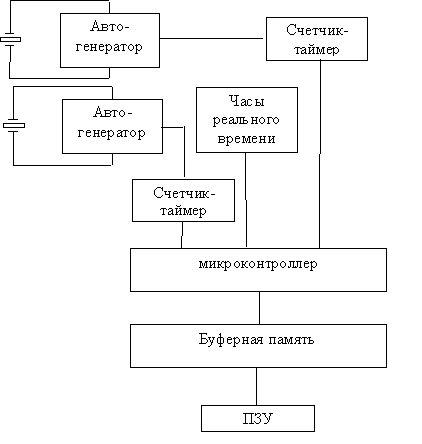
\includegraphics [scale=0.7] {ARV_regScheme.png}
  \caption{Структурная схема регистратора датчика придонного давления и температуры АРВ-К}
  \label{img:ARV_regScheme}
\end{figure}
\FloatBarrier

Все основные характеристики различных моделей автономного регистратора волнения представлены в табл. \ref{tbl:charact}

\LTXtable{\textwidth}{tblCharactCut}

Для передачи данных с датчиков на персональный компьютер используется последовательный интерфейс RS–232. Полученные данные подвергаются первичной обработке – преобразованию девиации частоты автогенератора в значения температуры воды и давления.

\subsection{Постановка АРВ-К: основные преимущества и недостатки притопленных измерителей волнения}\label{AppendexA_post}

Притопленные измерители волнения используются в ИМГиГ ДВО РАН для проведения длительных наблюдений за колебаниями уровня моря в прибрежной зоне с помощью автономных регистраторов волнения. Схема такой постановки приведена на рис. \ref{img:setSensor_3}.

Одним из наиболее существенных недостатков подповерхностных БС является сложность поиска аппаратуры, закрепленной на якоре таких буев. Проблема решается просто при использовании акустических размыкателей, но их цена достигает стоимости самой измерительной аппаратуры и поэтому в мелководной шельфовой зоне нами использовались варианты постановок с оттяжками - (донными) перемычками из плавучего полипропиленового каната, за которые затем вытраливали аппаратуру.

\begin{figure} [h]
  \center
  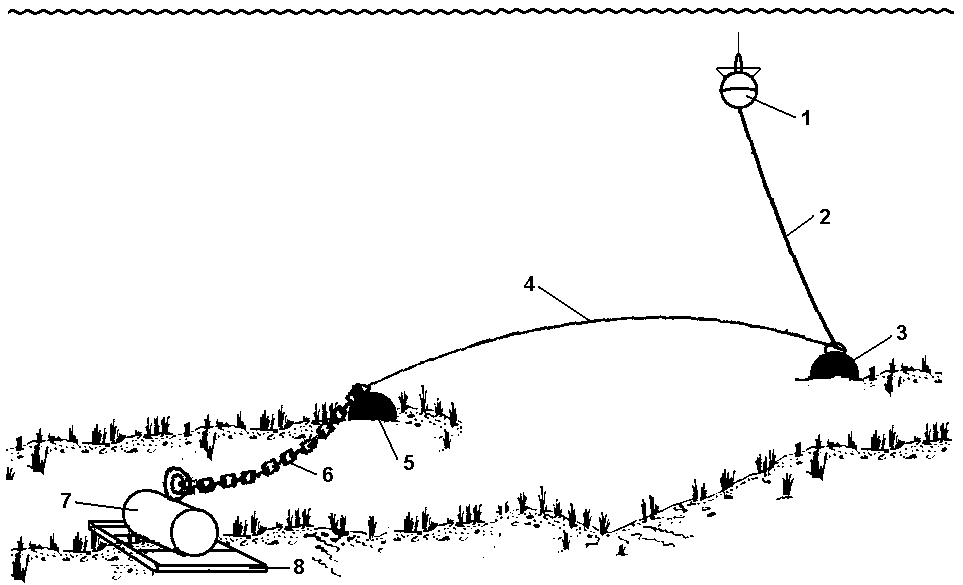
\includegraphics [width=0.7\linewidth] {setSensor_3.png}
  \caption{Схема постановки автономного регистратора волнения с ис-пользованием притопленной буйковой станции с двумя якорями. 1 -- притопленный буй; 2 -- буйреп;  3,5 -– якоря; 4 -– плавучий полипропиленовый канат (донная перемычка); 6 –- цепь; 7 –- АРВ; 8 –- рама.}
  \label{img:setSensor_3}
\end{figure}
\FloatBarrier


Кроме того, притопленный измеритель волнения исключает возможность измерения метеорологических элементов над поверхностью океана, и улучшение качества измерений путем заглубления плавучести измерителя волнения под поверхностью океана обходится ценой потери данных в наиболее динамичном верхнем слое океана и в приводном слое атмосферы.

Другим недостатком притопленных измерителей волнения является невозможность установки приборов на заданные горизонты, что очень важно изучения внутренних волн и совместного анализа данных на различных горизонтах. Связано это с тем, что имеется большие неточности при определении заглубления буя, которое в значительной мере зависит от рельефа дна. Вследствие этого заглубление несущего буя и горизонты погружения приборов оказывается смещенным относительно заданных на величину отклонения фактической глубины места постановки измерителя волнения от расчетной, в то время как для поверхностных АБ отклонение фактической глубины постановки от расчетной отражается лишь на величине притравки буйрепа, а не горизонтах погружения приборов, так как несущий буй всегда находится на поверхности океана. По данным работы \cite{sensor_berto} на американских подповерхностных станциях отклонения от требуемых горизонтов иногда превышали 100 м.

Еще одним весьма существенным недостатком подповерхностных измерителей волнения является изменение величин заглубления притопленного несущего буя, что особенно при знакопеременных приливных течениях приводит к вертикальным перемещениям приборов. При этом возможен значительный горизонтальный снос приборов и  осложняется их поиск \cite{sensor_fomin}.

\section{Система регистрации волнения в режиме реального времени} \label{AppendixA_Online}
Для организации связи комплекса с сервером мониторинга, необходим стабильный интернет-канал, м. Свободный обладает слабым покрытием сотовой связью. Поэтому для увеличения стабильности сигнала была применена направленная антенна, ориентированная в сторону сотовой вышки, а также промышленный модем, обеспечивающий стабильный прием сигнала сотовой станции. Как выяснилось в процессе работы с ними, модем обладает существенно большей стоимостью по сравнению с бытовыми GPRS-адаптерами, но в нем отсутствует недостаток, выявленный при работе с бытовыми адаптерами. Бытовые GPRS-модемы, комплексно реализуемые сотовыми компаниями, не держат постоянного подключения к интернету более полутора суток. Для установления соединения после подобного разрыва требуется не просто его включение-выключение, а снятие напряжения с USB порта, что вызывает большие трудности. Промышленные же модемы гарантируют постоянное соединение в течение долгого времени.

Схема блока регистрации, предварительной обработки и передачи данных  приведена на рис. \ref{img:electricScheme}
\begin{figure} [h]
  \center
  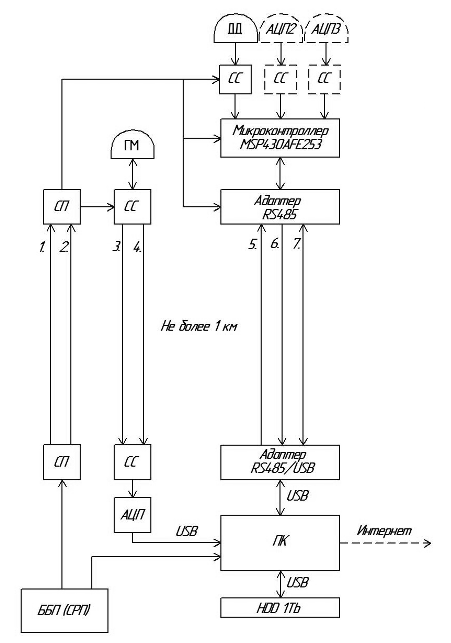
\includegraphics [scale=0.7] {electricScheme.png}
  \caption{Схема блока регистрации, предварительной обработки и передачи данных}
  \label{img:electricScheme}
\end{figure}
\FloatBarrier

Опишем подробнее каждый из элементов, представленных на рис. \ref{img:electicScheme}.
\begin{enumerate}
  \item ДД – датчик давления (опрос с периодичностью 5 – 10 ГЦ на выбор);
  \item АЦП2, АЦП3 – возможность подключить еще аналоговые датчики с такой же периодичностью опроса;
  \item СС-схема согласования;
  \item MSP430AFE253 – микроконтроллер с 3 канальным 24 битным сигма-дельта АЦП с дифференциальными входами;
  \item ГМ – гидрофонный модуль;
  \item СП – схема питания;
  \item ББП – блок бесперебойного питания;
  \item СРП – схема резервного питания;
  \item АЦП – аналога цифровой преобразователь;
  \item ПК – персональный компьютер;
  \item HDD – жесткий диск на 1 терабайт (при частоте дискретизации записи с ГМ 50к его хватит приблизительно на 117 дней);
  \item Интернет – возможен как спутниковый канал передачи данных, так и сотовый.
\end{enumerate}

Датчик давления подключается к комплексу посредством соединения схемой согласования с микроконтроллером MSP430AFE253, который обеспечивает предварительную обработку аналогового сигнала с датчика давления, кроме того еще позволяет дополнительно подключать другие аналоговые датчики, такие как датчики температуры, солености, электропроводности и т.д.

Данный микроконтроллер зарекомендовал себя, как надёжное устройство, он обеспечивает длительную работу устройств в портативных применениях за счет гибкой системы энергосбережения, позволяя динамически переключаться между пятью уровнями производительности, снижая энергопотребление приложения в те моменты, когда оно не активно и возвращаться снова в активный режим со скоростью менее 1мкс. В активном режиме микроконтроллер потребляет 220 мкА на 1 МГц, в спящем режиме 0,5 мкА на 1 МГц при напряжении питания 2,2 В. Еще одной важной отличительной особенностью этого микроконтроллера является наличие модуля SD24-A, содержащего три независимых 24-битных сигма-дельта АЦП и генератор опорного напряжения. Каждый АЦП содержит три мультиплексированных дифференциальных входа. Один из входов используется для подключения внешних источников сигнала, два других канала каждого АЦП подключены к терморезистору для оценки температуры микроконтроллера и делителю напряжения питания. Аналого-цифровые преобразователи модуля SD24-A построены на базе сигма-дельта модулятора второго порядка и цифровых децимирующих фильтров. Коэффициент децимации может принимать значения до 1024. В случае необходимости, дополнительная децимация может быть реализована программно. В зависимости от выбранного коэффициента децимации, разрядность результата преобразования составляет от 15 до 30 бит. По умолчанию установлен коэффициент децимации 256, что обеспечивает 24-битный результат на выходе цифрового фильтра. Встроенный опорный генератор АЦП выдает напряжение 1,2 В. Этот сигнал может быть выведен на вывод VREF микроконтроллера. На этот же самый вывод подается опорное напряжение при использовании внешнего генератора. Несколько аналого-цифровых преобразователей могут быть синхронизированы между собой для осуществления одновременного захвата внешних сигналов. Каждый из преобразователей содержит встроенный усилитель с цифровым управлением и коэффициентом усиления до 32. Также микроконтроллер содержит 16-битный аппаратный умножитель, сторожевой таймер, способный работать в режиме интервального таймера, 16-битный таймер общего применения с тремя регистрами захвата сравнения и универсальный последовательный интерфейс USART, конфигурируемый как UART, либо SPI.

Данный контроллер посредством адаптеров RS485/USB подключается к персональному компьютеру, где происходит предварительная обработка отсчетов, посылаемых микроконтроллером. В соответствие с этими алгоритмами обработки, был разработан и отлажен специализированный программный комплекс, реализованный на Delphi со вставками ассемблерного кода.


\chapter{название второго приложения} \label{AppendixB}


Даньелл (Daniell) предложил сглаживать быстрые флуктуации выборочного спектра путем усреднения по соседним частотам спектра. Данный метод, называемый периодограммой Даньелла, сводится к вычислению свертки периодограммы со сглаживающей функцией. В методе Бартлетта (Bartlett) анализируемый сигнал делится на неперекрывающиеся сегменты, для каждого сегмента вычисляется периодограмма и затем эти периодограммы усредняются. Если корреляционная функция сигнала на длительности сегмента затухает до пренебрежимо малых значений, то периодограммы отдельных сегментов можно считать независимыми. В этом случае дисперсия периодограммы Бартлетта обратно пропорциональна числу используемых сегментов, однако с ростом числа сегментов при фиксированном общем числе отсчетов сигнала падает спектральное разрешение (за счет того, что сегменты становятся короче).

Уэлч (Welch) внес в метод Бартлетта два усовершенствования: использование весовой функции и разбиение сигнала на перекрывающиеся фрагменты. Применение весовой функции позволяет ослабить растекание спектра и уменьшить смещение получаемой оценки спектра плотности мощности ценой незначительного ухудшения разрешающей способности. Перекрытие сегментов введено для того, чтобы увеличить их число и уменьшить дисперсию оценки. Метод Уэлча, согласно [Марпл--мл., 1990], является наиболее популярным периодограммным методом спектрального анализа.

 \section{Исходный код программы для выделения волн}\label{AppendixB1}
%\lstinputlisting{SignificantHeight_AppCode.cpp}